\chapter{アプリケーション例}
\$Vを利用したアプリケーション例を本章において示す.
\$Vは少ない学習データにおいて,高い認識率及び識別性能を示すため,ユーザ定義ジェスチャを利用したアプリケーションを開発することができる.
また,同じ形状及び書き順の手書きジェスチャを大きさ,向き,位置に関して識別可能であるため,それらを利用したアプリケーション例を示す.

\section{手書きジェスチャを利用したアプリケーション開発ツールキット}
まず,ユーザは,入力として用いたい手書きジェスチャを実際に手書きジェスチャを入力する端末を用いて学習データとして追加していく~(図\ref{fig:flow}a).
すると,\$Vが実装された本ツールキットは,追加された学習データを自動的にジェスチャグループに分類し,それぞれのジェスチャグループごとに,大きさ,向き,位置の特徴量に対する最適な重みを自動計算する~(図\ref{fig:flow}b).
最後に,ユーザは,あるアプリケーションにおける処理を実行するAppleScriptあるいはボタンと手書きジェスチャを対応付けることによって~(図\ref{fig:flow}c),手書きジェスチャを利用したアプリケーションを開発することができる.

\begin{figure} [h!]
	\begin{center}
		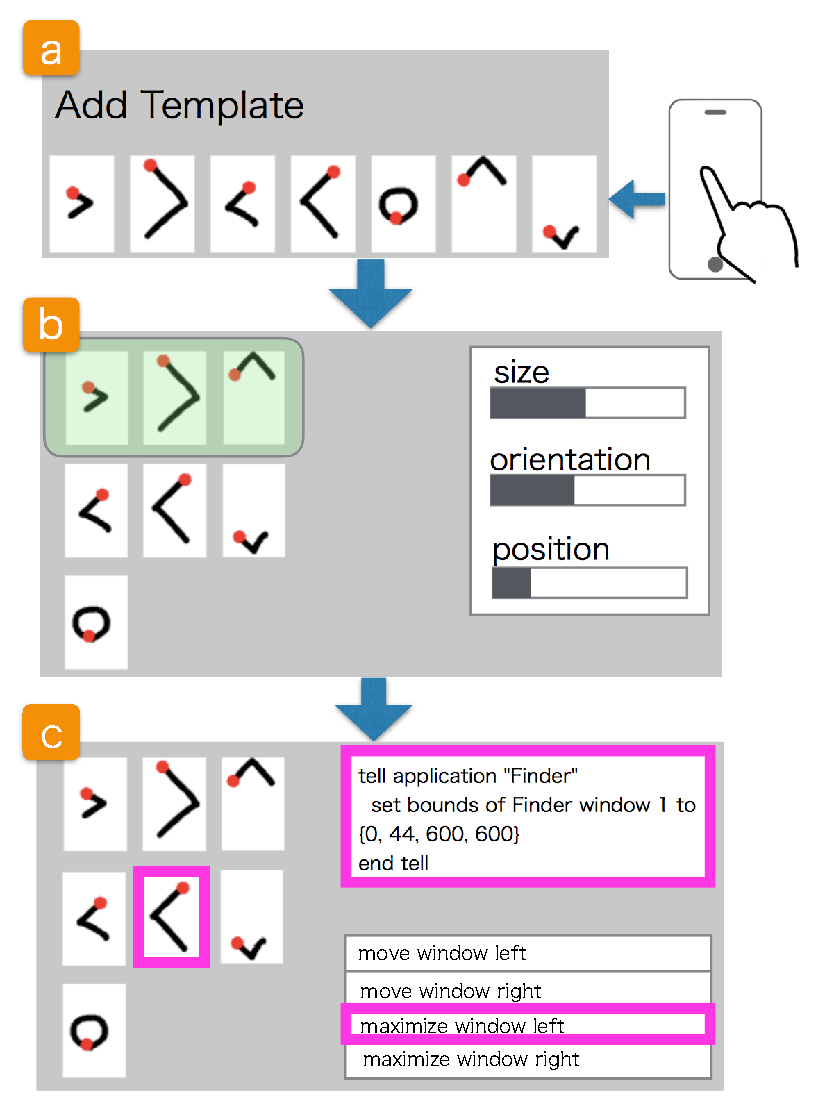
\includegraphics [width=0.8\hsize ]{img/flow.eps}
	\end{center}
	\caption{手書きジェスチャを利用したアプリケーション開発ツールキット.~(a)まず,ユーザはスマートフォンなどの手書きジェスチャを入力する端末を用いて学習データを追加し,~(b)\$Vが実装されたツールキットが追加された学習データを自動的にジェスチャグループに分類し,ジェスチャグループごとに重みを計算する.(c)最後にユーザはコマンドを割り当てる.}
	\label{fig:flow}
\end{figure}

このツールキット使うことによって,例えば,図\ref{fig:application}のようなメディアプレイヤを開発することができる.
このメディアプレイヤにおいて,再生,巻き戻し,前のメディア,次のメディアなどに対し,同じ書き順及び同じ形状の手書きジェスチャが割り当てられており~(図\ref{fig:application}A),それぞれ,大きさ,向きの違いが利用されている.ユーザはスマートフォンを手書きジェスチャの入力端末として用いることによって,PC上のメディアプレイヤを操作することが可能である~(図\ref{fig:application}B).
このようにして,大きさ,向き,位置の違いを利用することによって,より実際の動作に即した手書きジェスチャを割り当てることが可能となる.
また,大きさ,向き,位置の違いを利用できない場合と比べて,利用可能な手書きジェスチャの種類が大きく拡大し,アプリケーションユーザが入力として用いたい手書きジェスチャを考案しやすくなったと言える.

\begin{figure} [h!]
	\begin{center}
		\includegraphics [width=1.0\hsize ]{img/application.eps}
	\end{center}
	\caption{ツールキットを使って開発されたメディアプレイヤの例.~(a)アプリケーションのスクリーンショット,~(b)実際にスマートフォンを用いて入力している場面}
	\label{fig:application}
\end{figure}
